\section{Реализация и тестирование}
Предложенный алгоритм был реализован на платформе .NET как часть проекта YaccConstructor; основным языком разработки являлся F\#~\cite{FSharp}. Ранее в рамках проекта был реализован RNGLR-алгоритм и генератор управляющих таблиц анализа для него. Управляющие таблицы RNGLR-алгоритма переиспользуются, поэтому внесения изменений в генератор не потребовалось. Также были переиспользованы структуры данных для структурированного в виде графа стека GSS и компактного представления разбора SPPF. 

Алгоритм был протестирован на различных наборах тестов. Для каждого теста специфицировалась грамматика на языке YARD и в явном задавался граф конечного автомата, ребра которого были промаркированы лексемами эталонной грамматики. Полученный в результате работы алгоритма лес разбора печатался в файл и проверялся на корректность. Тесты можно разделить на две категории.
\begin{itemize}
  \item \emph{Регрессионные тесты} проверяющие, что предложенный алгоритм выдаёт те же результаты, что и RNGLR-алгоритм, на линейном входе (конечном автомате, принимающем единственную строку). В данный набор вошли все тесты, ранее использованные для тестирования работоспособности реализации RNGLR-алгоритма в проекте YaccConstructor. 
  \item \emph{Тесты на работоспособность}, проверяющие, что алгоритм строит корректное представление леса разбора всех корректных выражений из входного регулярного множества. Входные графы для данного набора тестов содержали как ветвления, так и циклы. Отдельно были рассмотрены случаи вложенных ветвлений и вложенных циклов. На всех тестах алгоритм генерировал корректный лес разбора, игнорируя некорректные относительно эталонной грамматики цепочки.
\end{itemize}

Замеры времени работы алгоритма проводились на машине со следующими техническими характеристиками: Intel(R) Core(TM) i7-4790 CPU @ 3.60GHz, RAM: 16.0~GB, процессор x64.

\subsection{Тестирование производительности}
Алгоритм был протестирован на нескольких сериях синтетических тестов, цель которых~--- убедиться в приемлемой производительности алгоритма на практически значимых входных данных. Анализ промышленного проекта по миграции базы данных с MS-SQL Server 2005 на Oraclе 11gR2 показал, что запросы часто формируются конкатенацией фрагментов, каждый из которых формируется с помощью ветвлений или циклов. Ниже приведена эталонная грамматика, использованная в этих тестах. 
$$
\begin{array}{crcl}
& start\_rule &::=& s \\
& s & ::= & s \mbox{\texttt{ PLUS }} \mbox{\texttt{n}}\\
& n & ::= & \mbox{\texttt{ONE | }} \mbox{\texttt{TWO | }} \mbox{\texttt{THREE | }} \mbox{\texttt{FOUR | }} \mbox{\texttt{FIVE | }} \mbox{\texttt{SIX | }} \mbox{\texttt{SEVEN}}
\end{array}
$$

Входные графы представляли собой конкатенацию базовых блоков. Каждая серия тестов характеризовалась тремя параметрами: 
\begin{itemize}
  \item $height$~--- количество ветвлений в базовом блоке;
  \item $length$~--- максимальное количество повторений базовых блоков;
  \item $isCycle$~--- наличие в базовом блоке циклов (если ложь, то используются базовые блоки, изображённые на рисунке~\ref{block}, если истина~--- то изображённые на рисунке~\ref{block_loop}).
\end{itemize}

\begin{figure}[h!]
 \centering
 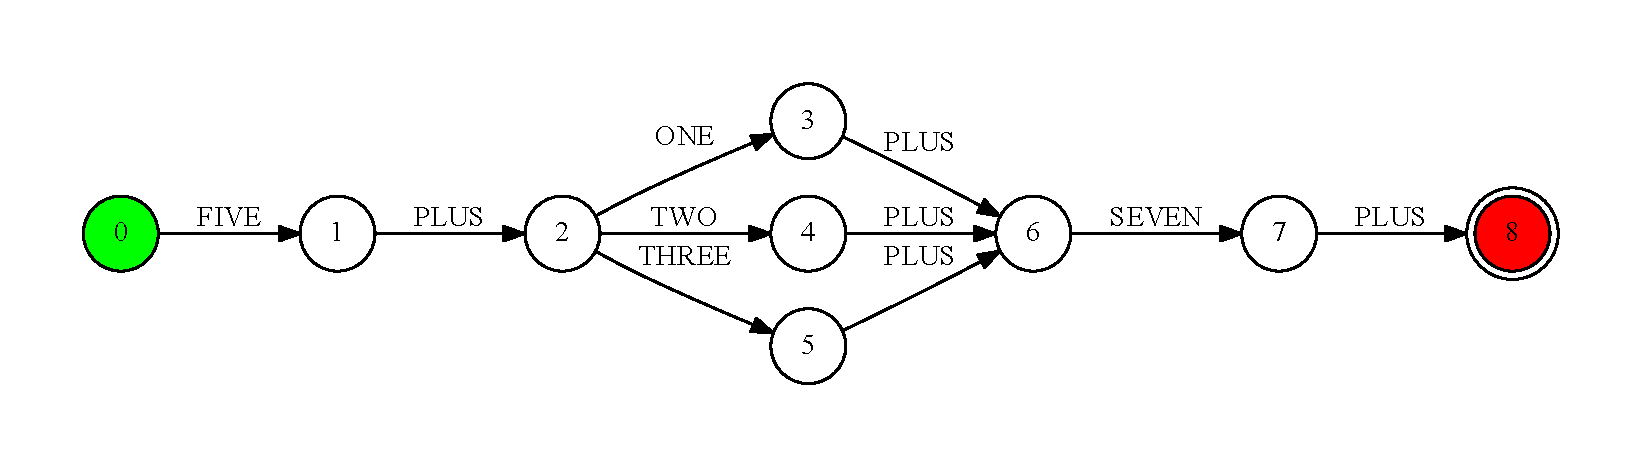
\includegraphics[width=15cm]{pics/block.pdf}
 \caption{Базовый блок без циклов при $length=3$}
 \label{block}
\end{figure}

\begin{figure}[h!]
 \centering
 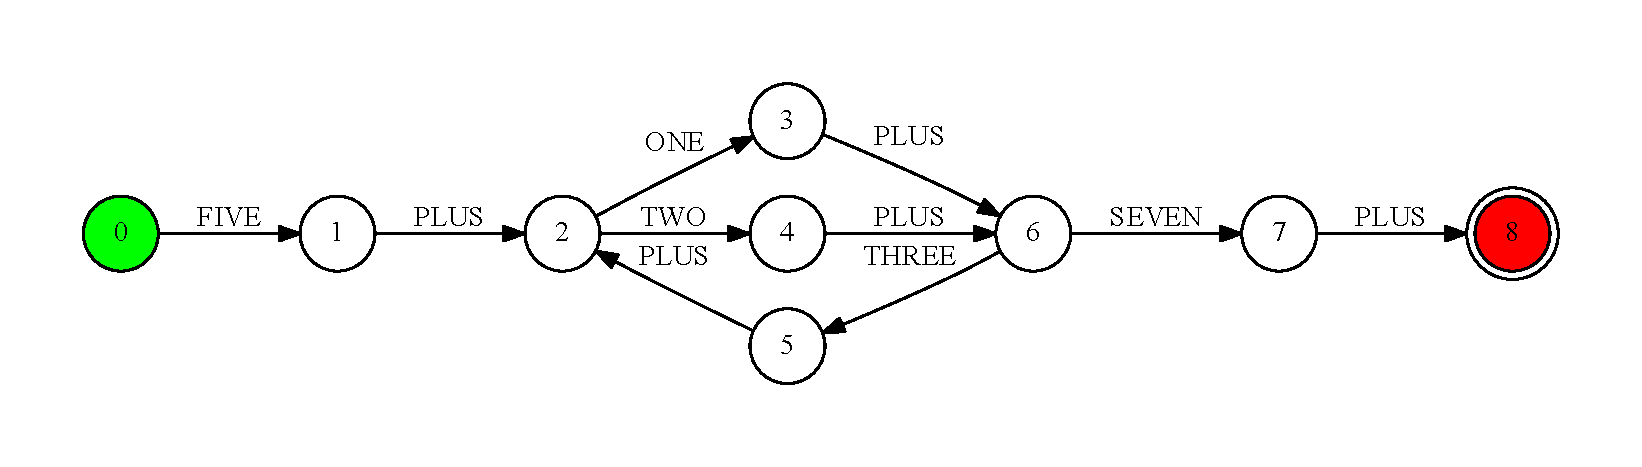
\includegraphics[width=15cm]{pics/block_loop.pdf}
 \caption{Базовый блок, содержащий цикл, при $length=3$}
 \label{block_loop}
\end{figure}

Каждая серия объединяет набор из $500$ тестов, каждый из которых содержит одинаковое количество ветвлений в базовом блоке, при этом количество повторений блока совпадает с порядковым номером теста ($length=i$ для $i$-того теста). Для каждого теста измерялось время, затраченное на синтаксический анализ. Измерения проводились 10 раз, после чего усреднялись, при этом выбросы не учитывались. График, представленный на рисунке~\ref{diffheights}, иллюстрирует зависимость времени, затрачиваемого на синтаксический анализ, от количества повторения базового блока и количества ветвлений в каждом из них. Можно заметить, что продолжительность анализа растёт линейно, в зависимости от размера входного графа. График на рисунке~\ref{CycleVsLinear} демонстрирует, что наличие циклов в графе увеличивает продолжительность анализа, при этом зависимость времени от размера графа остаётся линейной. 
\begin{figure}[h!]
 \centering
 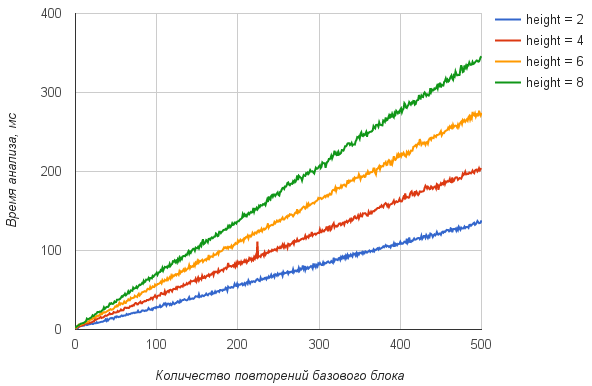
\includegraphics[width=15cm]{pics/diffheights.png}
 \caption{Зависимость времени работы алгоритма от размера входного графа при $isCycle=false$}
 \label{diffheights}
\end{figure}
\begin{figure}[h!]
 \centering
 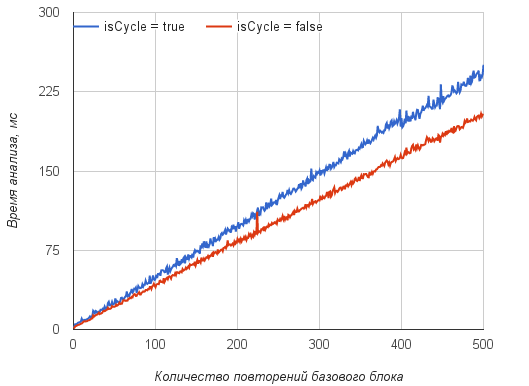
\includegraphics[width=15cm]{pics/heigh4.png}
 \caption{Зависимость времени работы алгоритма от размера входного графа и наличия в нем циклов при $height=4$}
 \label{CycleVsLinear}
\end{figure}

\clearpage
\subsection{Тестирование на реальных данных}
Алгоритм был протестирован на наборе данных, взятых из промышленного проекта по миграции базы данных с MS-SQL Server 2005 на Oraclе 11gR2. Система содержала около 2,6 миллионов строк кода, 2430 динамических запросов, из которых больше 75\% могут принимать более одного значения. Реализация алгоритма была внедрена в проект по миграции, заменив ранее используемую версию алгоритма синтаксического анализа. Алгоритм запускался на данной системе 10 раз, время анализа усреднялось. 

Алгоритм успешно завершил работу на 2188 входных графах, аппроксимирующих множества значений запросов. Ручная проверка входных графов, на которых алгоритм завершался с ошибкой, показала, что они действительно не содержали ни одного корректного в эталонном языке выражения. Причиной этого стала либо некорректная работа токенизатора, либо наличие в выражениях конструкций, не поддержанных в существующей грамматике. Дальнейшие значения приводятся только для графов, которые удалось проанализировать. 604 из этих графов содержали ровно один путь и анализировалось не более 1 миллисекунды. Общее время синтаксического анализа составило порядка 27 минут, из них 13 минут было затрачено на разбор графов, не содержащих ни одного корректного выражения. В среднем один такой граф анализировался 386 миллисекунд. На разбор 1790 графов ушло не более 10 миллисекунд. На анализ двух графов было затрачено более 2 минут: 152,215 и 151,793 секунд соответственно. Первый граф содержал 2454 вершин и 54335 рёбер, второй~--- 2212 вершин и 106020 рёбер. Распределение входных графов по промежуткам времени, затраченным на анализ, приведено на графике на рисунке~\ref{distr}.

Тестирование на реальных данных показало, что алгоритм применим для синтаксического анализа регулярной аппроксимации множества значений динамически формируемого выражения.

\begin{figure}[H]
  \centering
 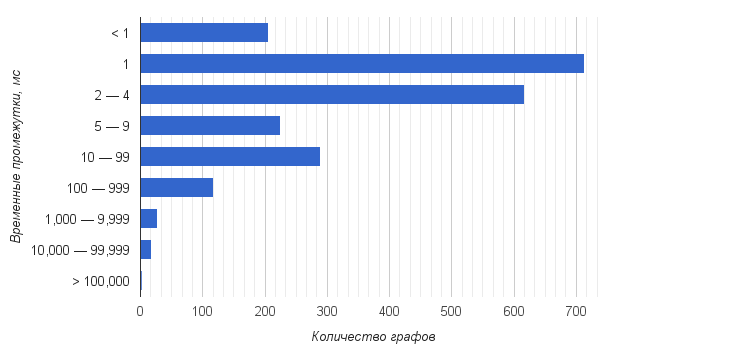
\includegraphics[width=15cm]{pics/distr.png}
 \caption{Распределение запросов по времени анализа}
 \label{distr}
\end{figure}